% !TeX encoding = UTF-8
%
% Grafische Oberflächen:
%


%
% Grafische Oberflächen starten auf eigener Seite.
%
\clearpage


\section{Grafische Oberfl{"a}chen}
\label{NU:GO}~\\

\subsection*{\underline{Pflicht-Oberflächen:}}

\begin{ids}{\gls{PGO}}

	\id[0010] Ein Hauptmenü mit Auswahl zum "challenge" Modus und zum "creative" Modus.
	\id[0020] Ein Menü für der "creativ" Modus um sich zwischen dem erstellen eines neuen Knotens, einer neuen Herausforderung und dem Laden eines Knotens zu entscheiden.
	\id[0030] Ein Men{"u} in dem man sich aussuchen kann, welcher Knoten geladen werden soll.
	\id[0040] Ein Men{"u} in dem man eine neue Herausforderung zusammenstellt.
	\id[0050] Ein Men{"u} in dem man eine Herausforderung zu spielen ausw{"a}hlen kann.
	\id[1010] Ein Editor, in dem man den Knoten bearbeitet.
	\id[1020] Im Editor /PGO\_1010/ eine Spielfl{"a}che in dem man den Knoten sieht und bearbeitet.
	\id[1030] Im Editor /PGO\_1010/ ein Pausenmen{"u}, in dem man im "creative" Modus speichern und in jedem Modus das bearbeiten beenden kann.
	\id[1040] Im Editor /PGO\_1010/ ein Zugang um ins Pausenmen{"u} /PGO\_1030/ zu gelangen.

\end{ids}

% ToDo: Refs (aber nur wenn noch Zeit) !!!

~\\


\subsection*{\underline{Optionale Oberflächen:}}

\begin{ids}{\gls{OGO}}

	\id[0010] Im Hauptmen{"u} /PGO\_0010/ eine Auswahl um die Credits anzuzeigen.
	\id[0020] Ein Men{"u} f{"u}r verschiedene Spieleinstellungen.
	\id[0030] Im Hauptmen{"u} /PGO\_0010/ eine Auswahl um zum Men{"u} f{"u}r Spieleinstellungen /OGO\_0020/ zu kommen.
	\id[0040] Im Einstellungsmen{"u} /OGO\_0020/ ein Untermen{"u} f{"u}r die Tastaturbelegung.
	\id[0050] Im Einstellungsmen{"u} /OGO\_0020/ ein Untermen{"u} f{"u}r grafische Einstellungen.
	\id[0060] Im Einstellungsmen{"u} /OGO\_0020/ ein Untermen{"u} f{"u}r audio Einstellungen.
	\id[0070] Im Einstellungsmen{"u} /OGO\_0020/ ein Untermen{"u} f{"u}r eine personaliesierte Farbpalette.
	\id[1010] Im Pausenmen{"u} /PGO\_1030/ ein Eintrag um das Einstellungsmen{"u} /OGO\_0020/ anzuzeigen.
	\id[1020] Ein Men{"u} f{"u}r verschiedene Render- und Exportfunktionen.
	\id[1030] Im Editor /PGO\_1010/ eine M{"o}glichkeit das Rendermen{"u} /OGO\_1020/ aufzurufen.
	\id[1040] /OGO\_1030/ ist nur im "crative" Modus und nach bestandener Herausforderung zugänglich.
\end{ids}


% ToDo: An sich wäre noch eine direkte Verlinkung auf die Grafiken and er entsprechenden Stelle gut.


\subsection*{\underline{Visualisierungen:}}
	\begin{figure}[h]
		\centering
	 	\includesvg[width = 0.95\textwidth]{menu}
	 	\caption{Hauptmen{"u}struktur beginnend mit /PGO\_0010/. Grau hinterlegtes ist Optional.}
	\end{figure}

	\begin{figure}[h]
		\centering
	 	\includesvg[width = 0.95\textwidth]{ingamemenu}
	 	\caption{Zugriffsm{"o}glichkeiten im Editor /PGO\_1010/. Grau hinterlegtes ist Optional. ~//
			1: Nur im "creative" Modus ~//
			2: Nur im "creative" Modus und nach bestandener Herausforderung}
	\end{figure}
	
	\begin{figure}[ht]
	  \centering
	  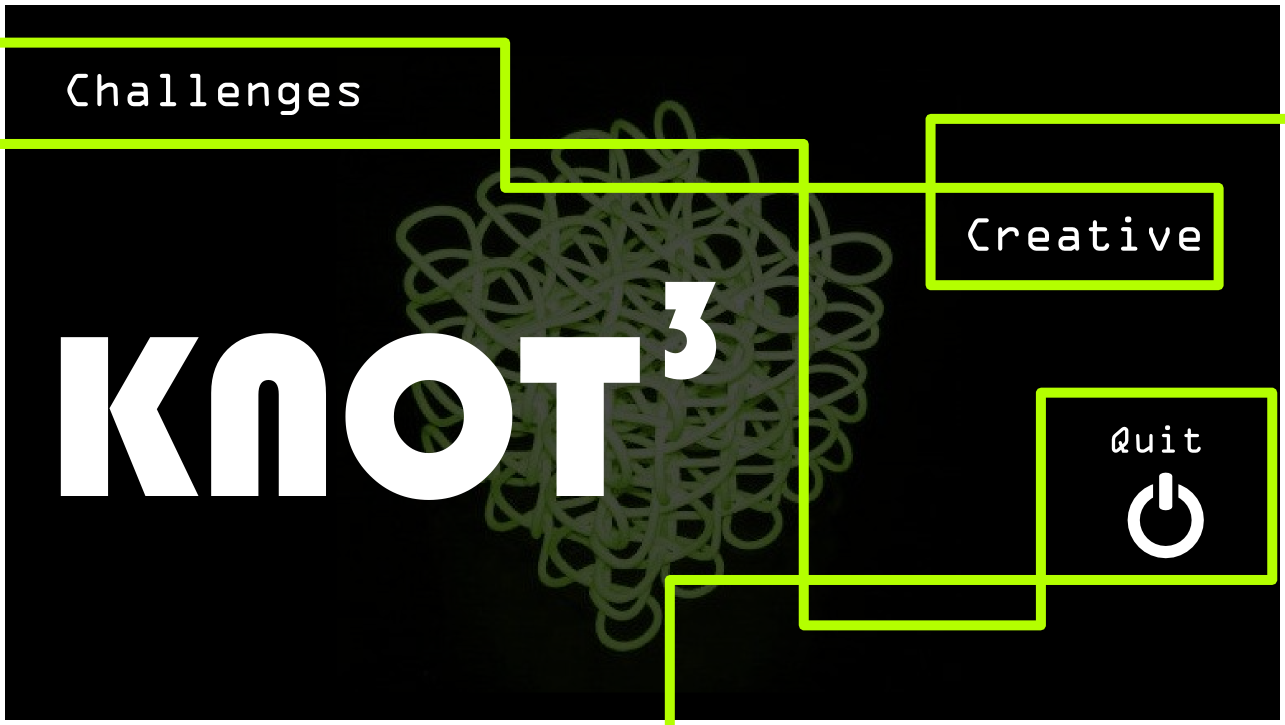
\includegraphics[width = 0.95\textwidth]{Inhalt/Nutzung/Grafiken/Grafische_Oberflaechen/01_Knot3-mainscreen.png}
	  \caption{Mögliches Hauptmenü /PGO\_0010/}
	\end{figure}

	\begin{figure}[ht]
	  \centering
	  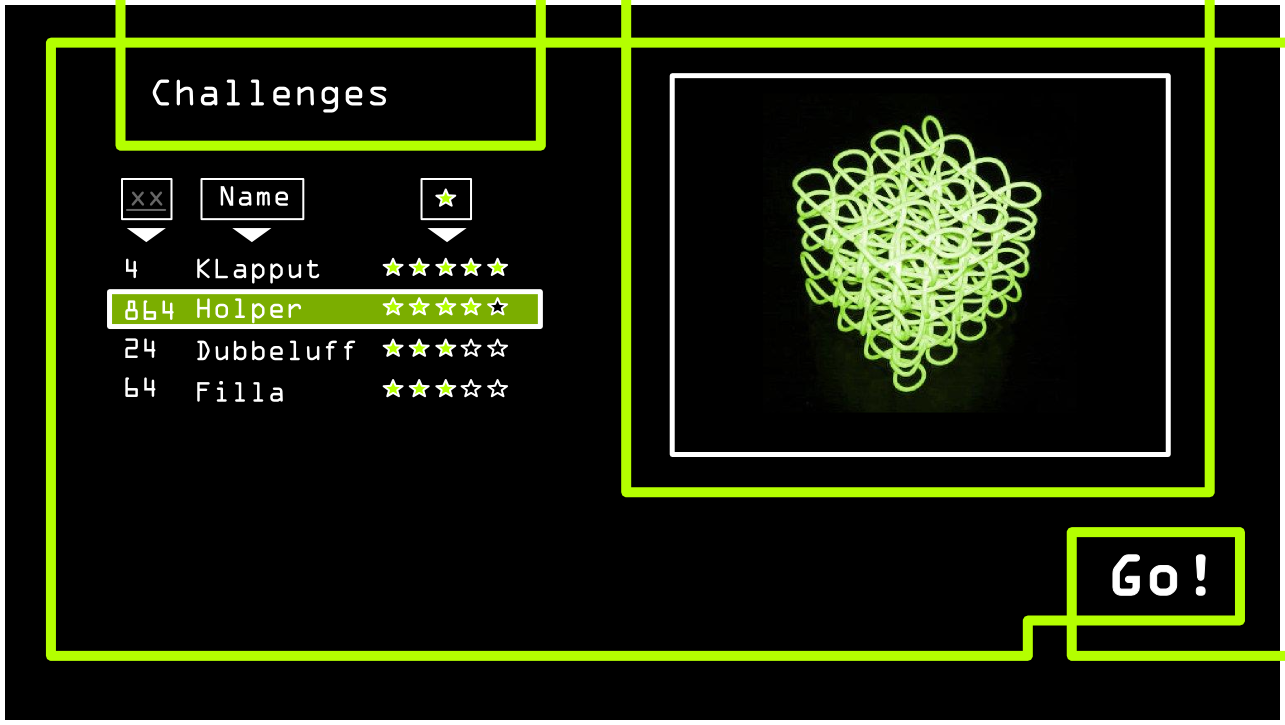
\includegraphics[width = 0.95\textwidth]{Inhalt/Nutzung/Grafiken/Grafische_Oberflaechen/04_Knot3-select-Challenge.png}
	  \caption{Auswahlmenü für die Herausforderungen /PGO\_0050/, mit Ausschnitt der Auswahlliste}
	\end{figure}
	
	\begin{figure}[ht]
	  \centering
	  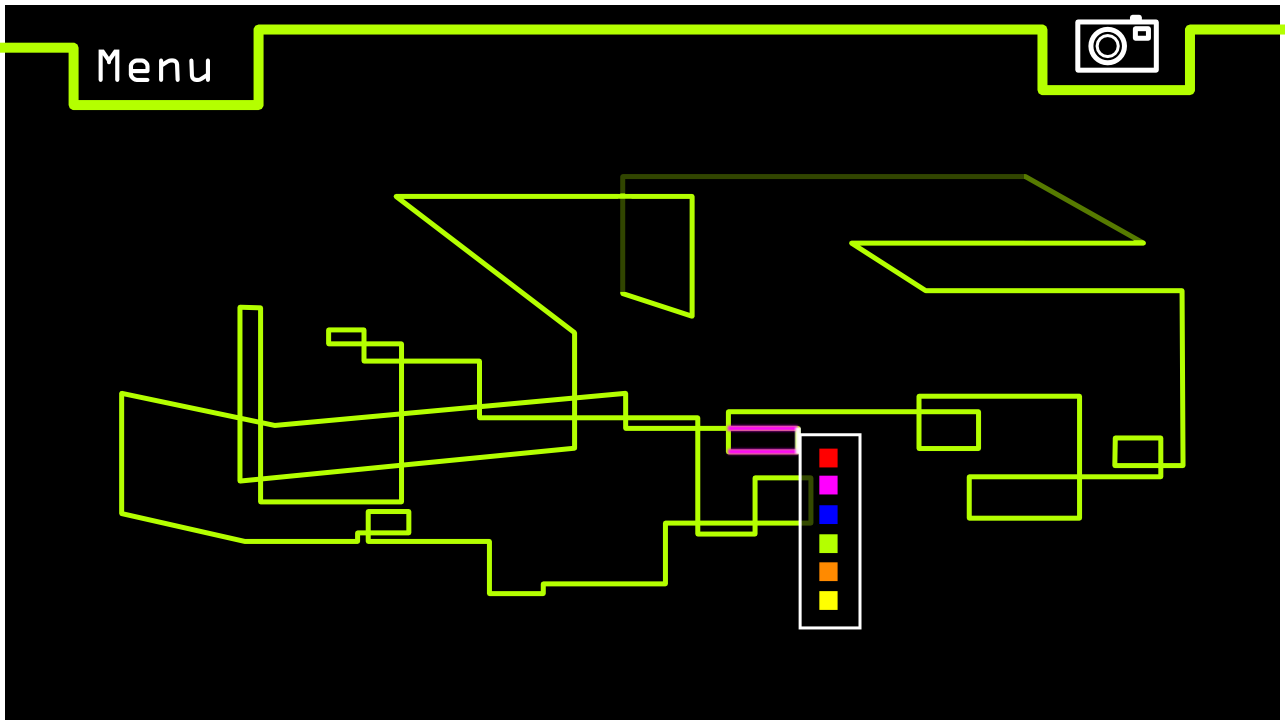
\includegraphics[width = 0.95\textwidth]{Inhalt/Nutzung/Grafiken/Grafische_Oberflaechen/05_Knot3-Colour-select.png}
	  \caption{Editoransicht /PGO\_1010/ mit geöffneter Farbauswahl zum Kanten einfärben /OFA\_200/.}
	\end{figure}
	
	\begin{figure}[ht]
	  \centering
	  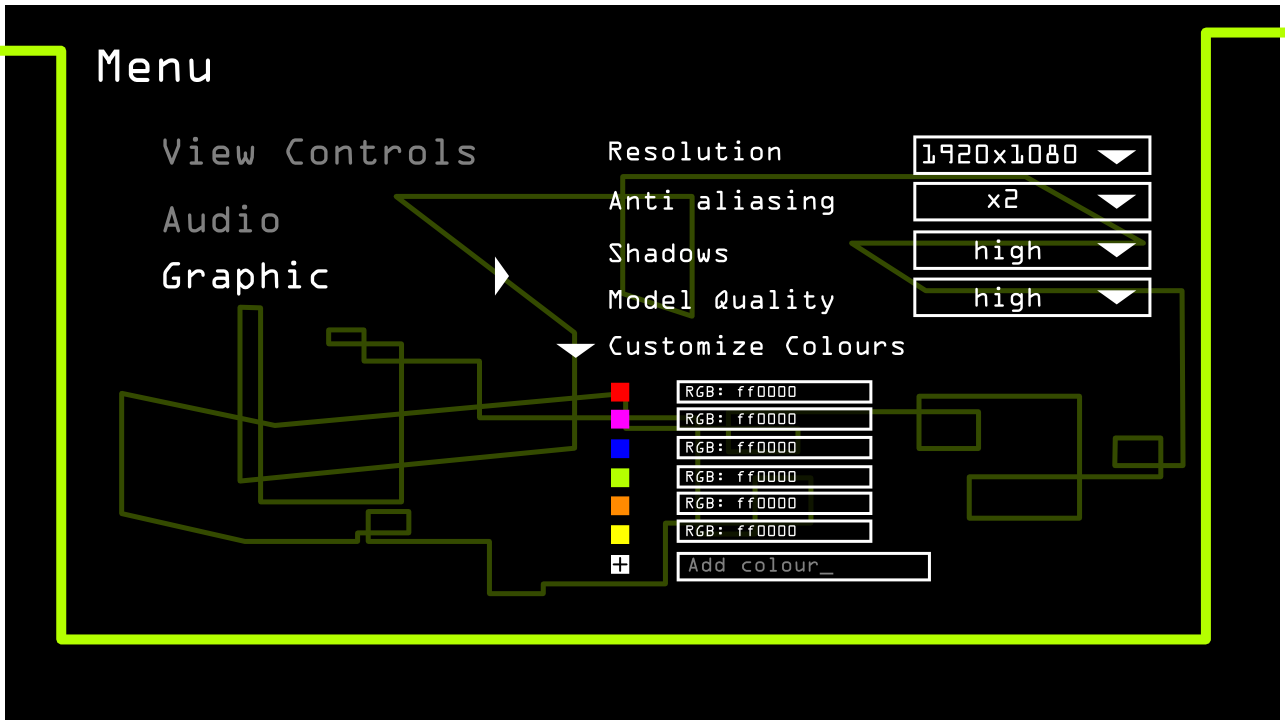
\includegraphics[width = 0.95\textwidth]{Inhalt/Nutzung/Grafiken/Grafische_Oberflaechen/08_Knot3-menu-graphics.png}
	  \caption{Mögliches Einstellungsmenü mit geöffnetem Untermenü für die Grafikeinstellungen. /OGO\_0020/ und /OGO\_0050/}
	\end{figure}

